\documentclass[12pt]{article}
\usepackage{fullpage}
\usepackage{hyperref}
\hypersetup{bookmarks=true,colorlinks=true,linkcolor=red,citecolor=blue,filecolor=magenta,urlcolor=cyan}
\usepackage{amsmath}
\usepackage{longtable}
\usepackage{booktabs}
\usepackage{caption}
\usepackage{graphics}
\title{Software Requirements Specification for Solar Water Heating Systems}
\author{Thulasi Jegatheesan}
\begin{document}
\maketitle
\tableofcontents
\newpage
\section{Reference Material}
\label{Sec:RM}
This section records information for easy reference.
\subsection{Table of Units}
\label{Sec:ToU}
The unit system used throughout is SI (Syst\`{e}me International d'Unit\'{e}s). In addition to the basic units, several derived units are also used. For each unit, the table lists the symbol, a description and the SI name.
\begin{longtable*}{l l}
\toprule
Symbol & Description
\\
\midrule
m & length (metre)
\\
kg & mass (kilogram)
\\
s & time (second)
\\
${}^{\circ}C$ & temperature (centigrade)
\\
J & energy (joule)
\\
W & power (watt)
\\
\bottomrule
\label{Table:ToU}
\end{longtable*}
\subsection{Table of Symbols}
\label{Sec:ToS}
The table that follows summarizes the symbols used in this document along with their units. The choice of symbols was made to be consistent with the heat transfer literature and with existing documentation for solar water heating systems. The symbols are listed in alphabetical order.
\begin{longtable*}{l l l}
\toprule
Symbol & Description & Units
\\
\midrule
$A_{C}$ & Coil surface area & $\text{m}^{2}$
\\
$A_{in}$ & Surface area over which heat is transferred in & $\text{m}^{2}$
\\
$A_{out}$ & Surface area over which heat is transferred out & $\text{m}^{2}$
\\
$C$ & Specific heat capacity & $\frac{\text{J}}{(\text{kg}{}^{\circ}C)}$
\\
$C^{L}$ & Specific heat capacity of a liquid & $\frac{\text{J}}{(\text{kg}{}^{\circ}C)}$
\\
$C_{W}$ & Specific heat capacity of water & $\frac{\text{J}}{(\text{kg}{}^{\circ}C)}$
\\
$D$ & Diameter of tank & m
\\
$g$ & Volumetric heat generation per unit volume & $\frac{\text{W}}{\text{m}^{2}}$
\\
$h$ & Convective heat transfer coefficient & $\frac{\text{W}}{(\text{m}^{2}{}^{\circ}C)}$
\\
$h_{C}$ & Convective heat transfer coefficient between coil and water & $\frac{\text{W}}{(\text{m}^{2}{}^{\circ}C)}$
\\
$L$ & Length of tank & m
\\
$m$ & Mass & kg
\\
$m_{W}$ & Mass of water & kg
\\
$q$ & Heat flux & $\frac{\text{W}}{\text{m}^{2}}$
\\
$q_{C}$ & Heat flux from coil & $\frac{\text{W}}{\text{m}^{2}}$
\\
$q_{in}$ & Heat flux in & $\frac{\text{W}}{\text{m}^{2}}$
\\
$q_{out}$ & Heat flux out & $\frac{\text{W}}{\text{m}^{2}}$
\\
$\mathbf{q}$ & Thermal flux vector & $\frac{\text{W}}{\text{m}^{2}}$
\\
$T$ & Temperature & ${}^{\circ}C$
\\
$T_{C}$ & Temperature of coil & ${}^{\circ}C$
\\
$T_{env}$ & Temperature of environment & ${}^{\circ}C$
\\
$T_{init}$ & Initial temperature & ${}^{\circ}C$
\\
$T_{W}$ & Temperature of water & ${}^{\circ}C$
\\
$t$ & Time & s
\\
$t_{final}$ & Time & s
\\
$V_{tank}$ & Volume of the cylindrical tank & $\text{m}^{3}$
\\
$V$ & Volume & $\text{m}^{3}$
\\
$V_{W}$ & Volume of water & $\text{m}^{3}$
\\
$\Delta{}T$ & Temperature difference & ${}^{\circ}C$
\\
$\rho{}$ & Density & $\frac{\text{kg}}{\text{m}^{3}}$
\\
$\rho{}_{W}$ & Density of water & $\frac{\text{kg}}{\text{m}^{3}}$
\\
$\tau{}$ & Dummy variable for integration over time & s
\\
\bottomrule
\label{Table:ToS}
\end{longtable*}
\subsection{Abbreviations and Acronyms}
\label{Sec:AaA}
\begin{longtable*}{l l}
\toprule
Symbol & Description
\\
\midrule
A & Assumption
\\
DD & Data Definition
\\
GD & General Definition
\\
GS & Goal Statement
\\
IM & Instance Model
\\
LC & Likely Change
\\
ODE & Ordinary Differential Equation
\\
PS & Physical System Description
\\
R & Requirement
\\
SRS & Software Requirements Specification
\\
SWHS & Solar Water Heating System
\\
T & Theoretical Model
\\
\bottomrule
\label{Table:AaA}
\end{longtable*}
\section{Introduction}
\label{Sec:I}
\subsection{Characteristics of Intended Reader}
\label{Sec:CoIR}
Reviewers of this documentation should have a strong knowledge in heat transfer theory. A third or fourth year Mechanical Engineering course on the topic is recommended. The reviewer should also have an understanding of differential equations, as typically covered in first and second year Calculus courses. The users of SWHS can have a lower level expertise, as explained in Section
\section{General System Description}
\label{Sec:GSD}
This section provides general information about the system, identifies the interfaces between the system and its environment, and describes the user characteristics and the system constraints.
\subsection{System Constraints}
\label{Sec:SC}
Figure~\ref{Figure::SC} shows the system context. A circle represents an external entity outside the software, the user in this case. A rectangle represents the software system itself (SWHS). Arrows are used to show the data flow between the section and its environment.
\begin{figure}
\begin{center}
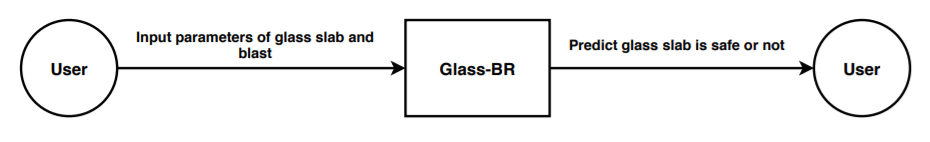
\includegraphics{SystemContextFigure.png}
\caption{Figure~\ref{Figure::SC}: System Context}
\label{Figure::SC}
\end{center}
\end{figure}
\section{Specific System Description}
\label{Sec:SSD}
This section first presents the problem description, which gives a high-level view of the problem to be solved. This is followed by the solution characteristics specification, which presents the assumptions, theories, definitions and finally the instance model (ODE) that models the solar water heating tank.
\subsection{Problem Description}
\label{Sec:PD}
SWHS is a computer program developed to investigate the heating of water in a solar water heating tank.
\subsubsection{Terminology and Definitions}
\label{Sec:TaD}
This subsection provides a list of terms that are used in subsequent sections and their meaning, with the purpose of reducing ambiguity and making it easier to correctly understand the requirements:
\begin{enumerate}
\item{Heat flux: the rate of heat energy transfer per unit area}
\item{Specific heat: heat capacity per unit mass}
\end{enumerate}
\subsubsection{Physical System Description}
\label{Sec:PSD}
The physical system of SWHS, as shown in Figure~\ref{Figure:Swht,whffco}, includes the following elements:
\begin{itemize}
\item[PS1:]Tank containing water
\item[PS2:]Heating coil at bottom of tank. ($q_{C}$ represents the heat flux from coil into the water.)
\end{itemize}
\begin{figure}
\begin{center}
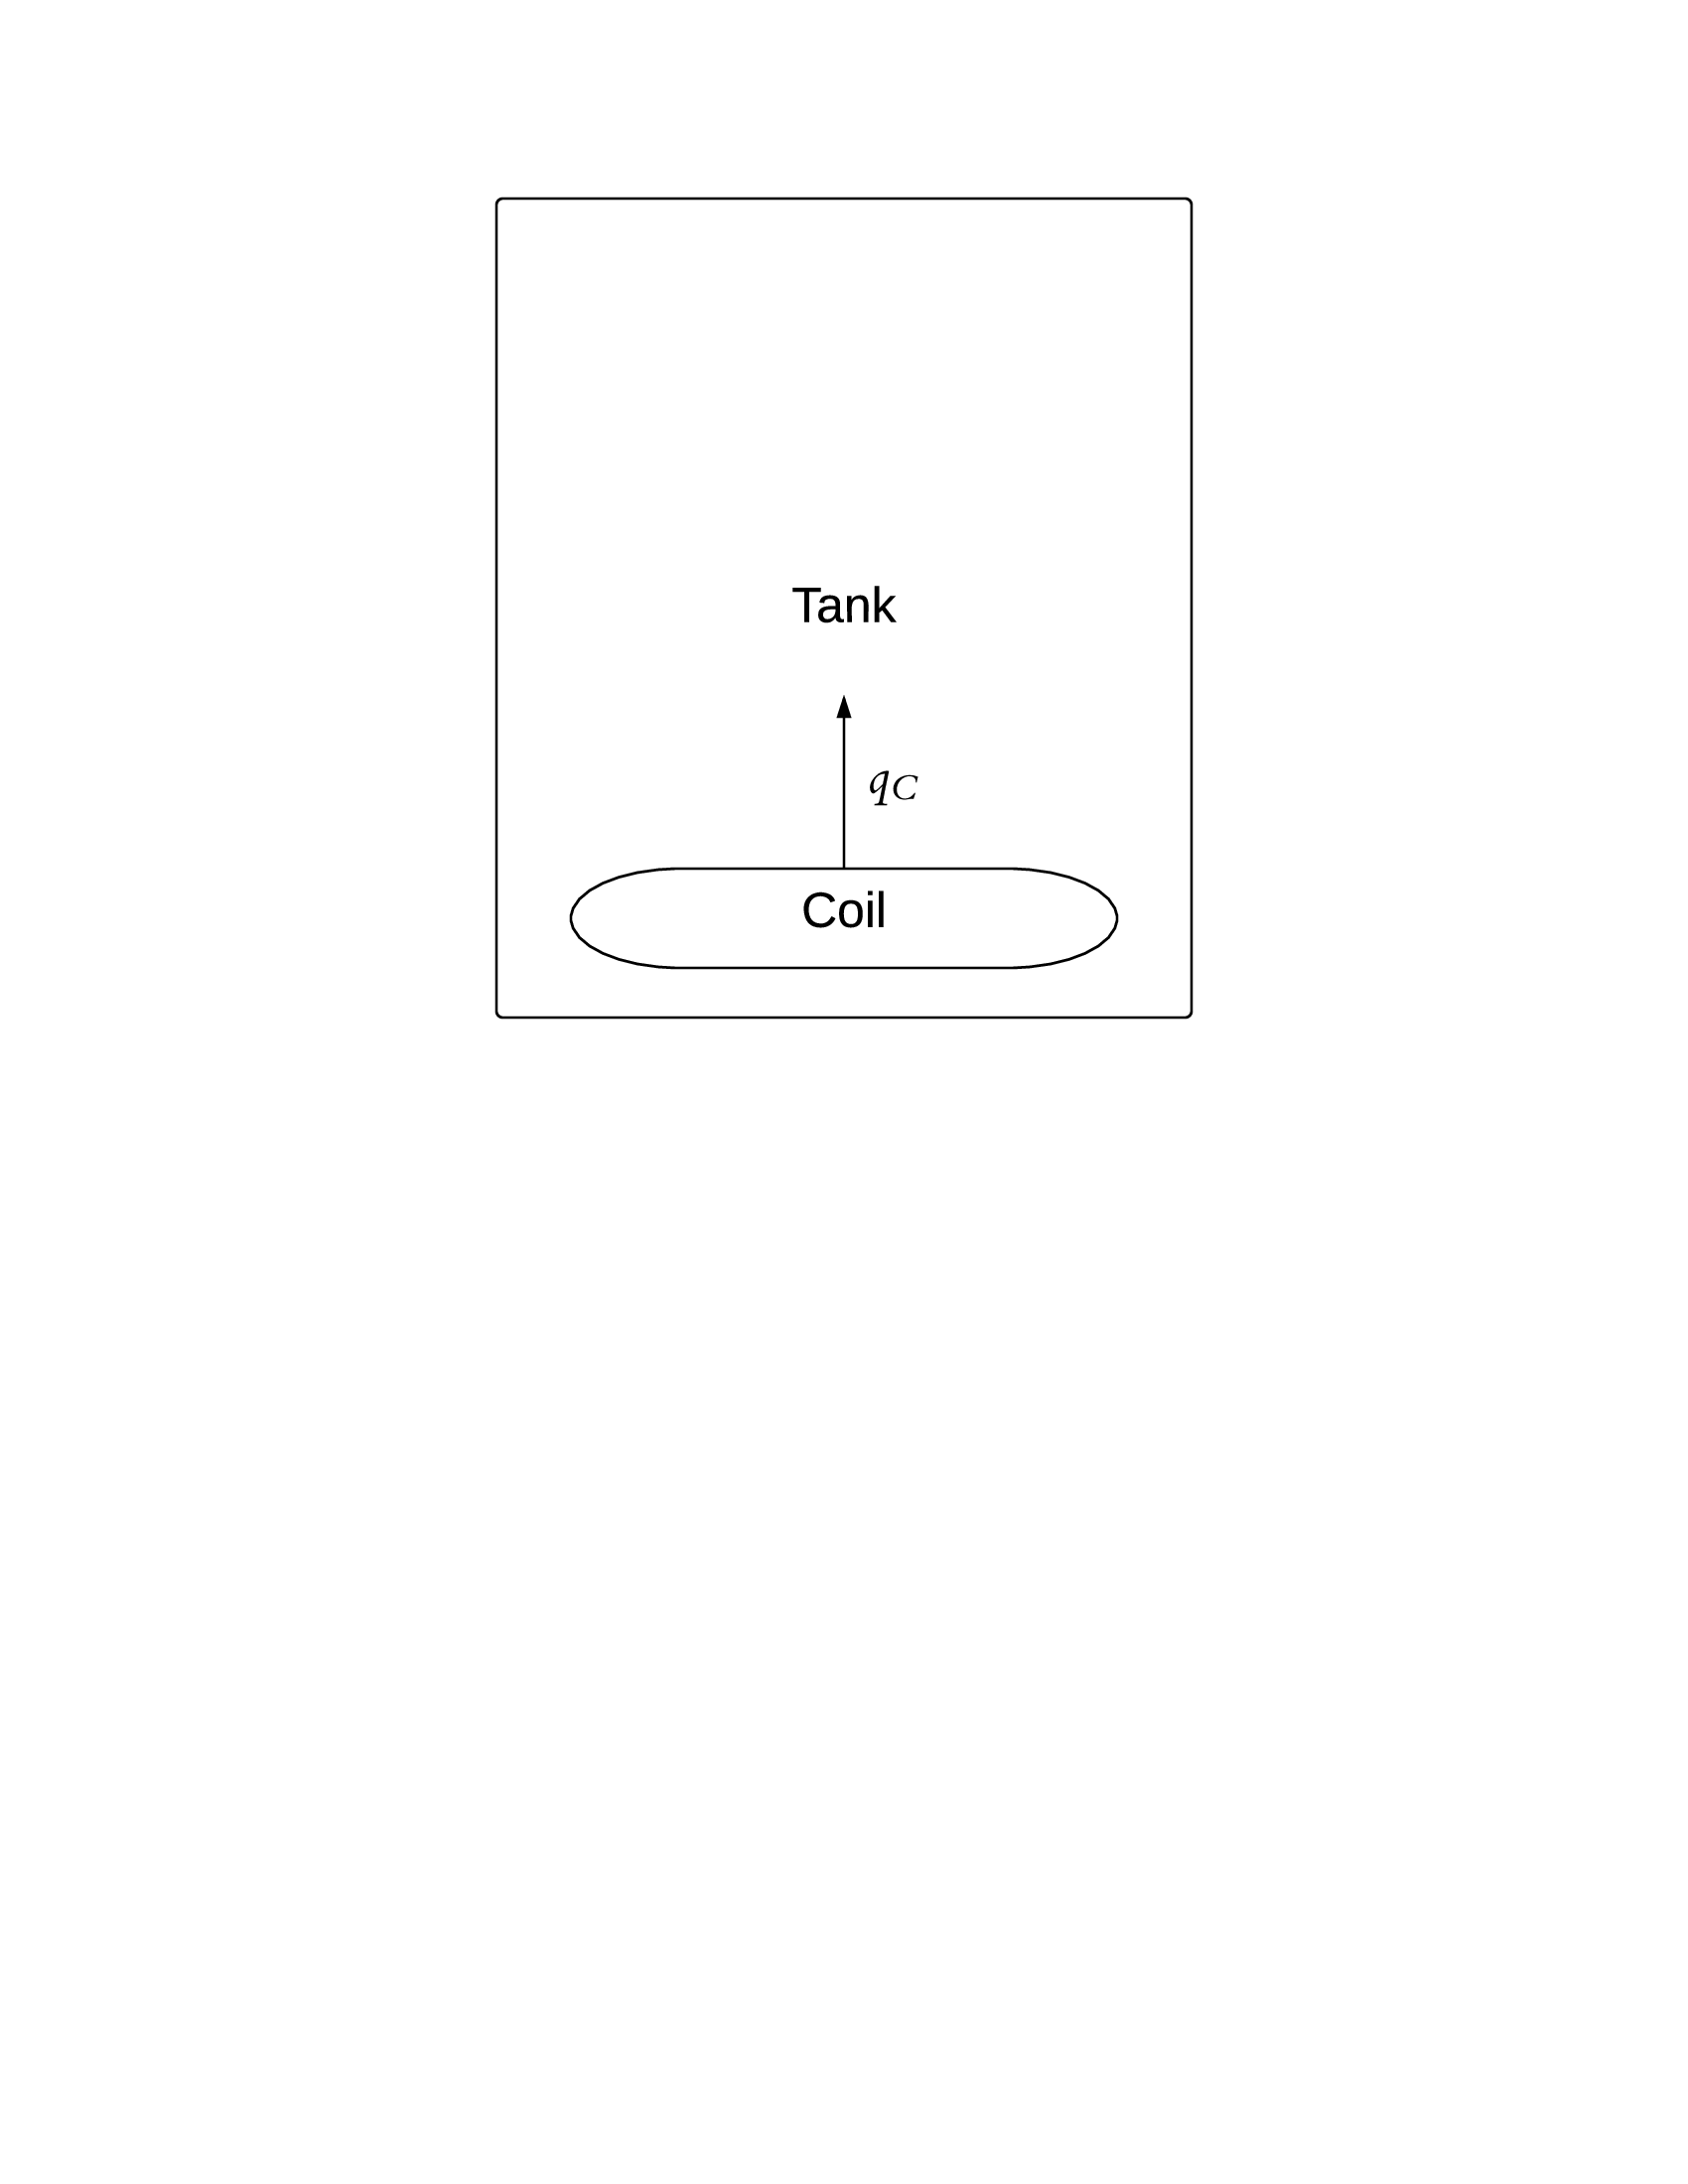
\includegraphics{TankWaterOnly.png}
\caption{Solar water heating tank, with heat flux from coil of $q_{C}$}
\label{Figure:Swht,whffco}
\end{center}
\end{figure}
\subsubsection{Goal Statements}
\label{Sec:GS}
Given the temperature of the coil, initial temperature of the water, and material properties, the goal statement is
\begin{itemize}
\item[GS1:]predict the temperature of water over time
\end{itemize}
\subsection{Solution Characteristics Specification}
\label{Sec:SCS}
The instance model (ODE) that governs SWHS is presented in . The information to understand the meaning of the instance model and its derivation is also presented, so that the instance model can be verified.
\subsubsection{Assumptions}
\label{Sec:A}
This section simplifies the original problem and helps in developing the theoretical model by filling in the missing information for the physical system. The numbers given in the square brackets refer to the theoretical model [T], general definition [GD], data definition [DD], instance model [IM], or likely change [LC], in which the respective assumption is used.
\subsubsection{Theoretical Models}
\label{Sec:TM}
This section focuses on the general equations and laws that SWHS is based on.
~\newline
\noindent \begin{minipage}{\textwidth}
\begin{tabular}{p{0.2\textwidth} p{0.73\textwidth}}
\toprule \textbf{Refname} & \textbf{T:t1consThermE}
\phantomsection 
\label{T:t1consThermE}
\\ \midrule \\
Label & Conservation of thermal energy
\\ \midrule \\
Equation & $-\nabla{}\cdot{}\mathbf{q}+g=\rho{}C\frac{\partial{}T}{\partial{}t}$
\\ \midrule \\
Description & This equation gives the conservation of energy for time varying heat transfer in a material of specific heat capacity $C$ and density $\rho{}$, where $\mathbf{q}$ is the thermal flux vector, $g$ is the volumetric heat generation, $T$ is the temperature, $t$ is time, and $\nabla{}$ is the gradient operator. For this equation to apply, other forms of energy, such as mechanical energy, are assumed to be negligible in the
\\ \bottomrule \end{tabular}
\end{minipage}\\
\subsubsection{General Definitions}
\label{Sec:GD}
This section collects the laws and equations that will be used in deriving the data definitions, which in turn are used to build the instance models.
\subsubsection{Data Definitions}
\label{Sec:DD}
This section collects and defines all the data needed to build the instance models.
\subsubsection{Instance Models}
\label{Sec:IM}
This section transforms the problem defined in Section~\ref{Sec:PD} into one which is expressed in mathematical terms. It uses concrete symbols defined in Section~\ref{Sec:DD} to replace the abstract symbols in the models identified in Section~\ref{Sec:TM} and Section~\ref{Sec:GD}.
\subsubsection{Data Constraints}
\label{Sec:DC}
Table~\ref{Table:T1IV} and Table~\ref{Table:T2OV} show the data constraints on the input and output variables, respectively. The column for physical constraints gives the physical limitations on the range of values that can be taken by the variable. The constraints are conservative, to give the user of the model the flexibility to experiment with unusual situations. The column of typical values is intended to provide a feel for a common scenario.
\begin{longtable}{l l l}
\toprule
Var & Physical Constraints & Typical Value
\\
\midrule
\bottomrule
\caption{Table 1: Input Variables}
\label{Table:T1IV}
\end{longtable}
\begin{longtable}{l l l}
\toprule
Var & Physical Constraints & Typical Value
\\
\midrule
\bottomrule
\caption{Table 2: Output Variables}
\label{Table:T2OV}
\end{longtable}
\end{document}
